\chapter{TỐI ƯU HÓA VÀ CẢI TIẾN MÔ HÌNH}
\label{chap:improve}

\section{Phân tích hạn chế của mô hình ban đầu}
\label{sec:limitations}

Mọi thí nghiệm trong mục này và các mục tiếp theo dùng đúng 5 fold, cùng tập mẫu kiểm định và cùng chỉ số như Chương~\ref{chap:models}, nên các kết quả so sánh được trực tiếp với nhau và với Bảng~\ref{tab:cv_summary}. Mọi lựa chọn chỉ dựa trên kiểm định chéo trong tập huấn luyện; tập kiểm tra năm 2010 chỉ được dùng ở Mục~\ref{sec:test}.

\subsection{Đường cong học tập}
Ở mỗi fold, mô hình được huấn luyện trên $n$ giờ gần nhất trước phần kiểm định (giữ nguyên khoảng đệm một tuần), với $n$ từ 1.000 đến cỡ phần huấn luyện của fold nhỏ nhất (khoảng 15.500 giờ), siêu tham số giữ như Chương~\ref{chap:models}. Hình~\ref{fig:learning_curve} cho thấy ba hành vi khác nhau:
\begin{itemize}
    \item Linear Regression: sai số huấn luyện tăng dần (0,340 lên 0,400 kWh ở $h = 1$) và gặp sai số kiểm định từ khoảng 8.000 mẫu, ở mức cao hơn mô hình cây. Đây là dạng điển hình của mô hình chưa khớp: thêm dữ liệu không giúp được nhiều vì mô hình thiếu khả năng biểu diễn.
    \item Random Forest: sai số trong mẫu gần như không đổi (0,22--0,24 kWh ở $h = 1$) vì mỗi cây luôn khớp sát dữ liệu của nó, còn sai số kiểm định giảm khi tăng dữ liệu (0,416 xuống 0,366 kWh ở $h = 1$; 0,565 xuống 0,497 kWh ở $h = 24$).
    \item XGBoost: với 1.000 mẫu, sai số trong mẫu chỉ 0,034 kWh trong khi sai số kiểm định là 0,444 kWh ($h = 1$), tức với ít dữ liệu, 400 cây độ sâu 6 gần như học thuộc dữ liệu; khoảng cách thu hẹp dần khi tăng dữ liệu.
\end{itemize}
Với hai mô hình cây, sai số kiểm định giảm nhanh đến khoảng 8.000 mẫu rồi gần như đi ngang (sai số của Linear Regression ở $h = 24$ dao động khi dữ liệu ít, nhưng cũng đi ngang từ 8.000 mẫu); ở $h = 24$, từ 8.000 đến khoảng 15.500 mẫu, Random Forest chỉ giảm từ 0,499 xuống 0,497 kWh và XGBoost từ 0,512 xuống 0,509 kWh. Như vậy thêm dữ liệu cùng loại khó cải thiện đáng kể; muốn giảm sai số cần cung cấp cho mô hình thông tin mới.

\begin{figure}[htbp]
    \centering
    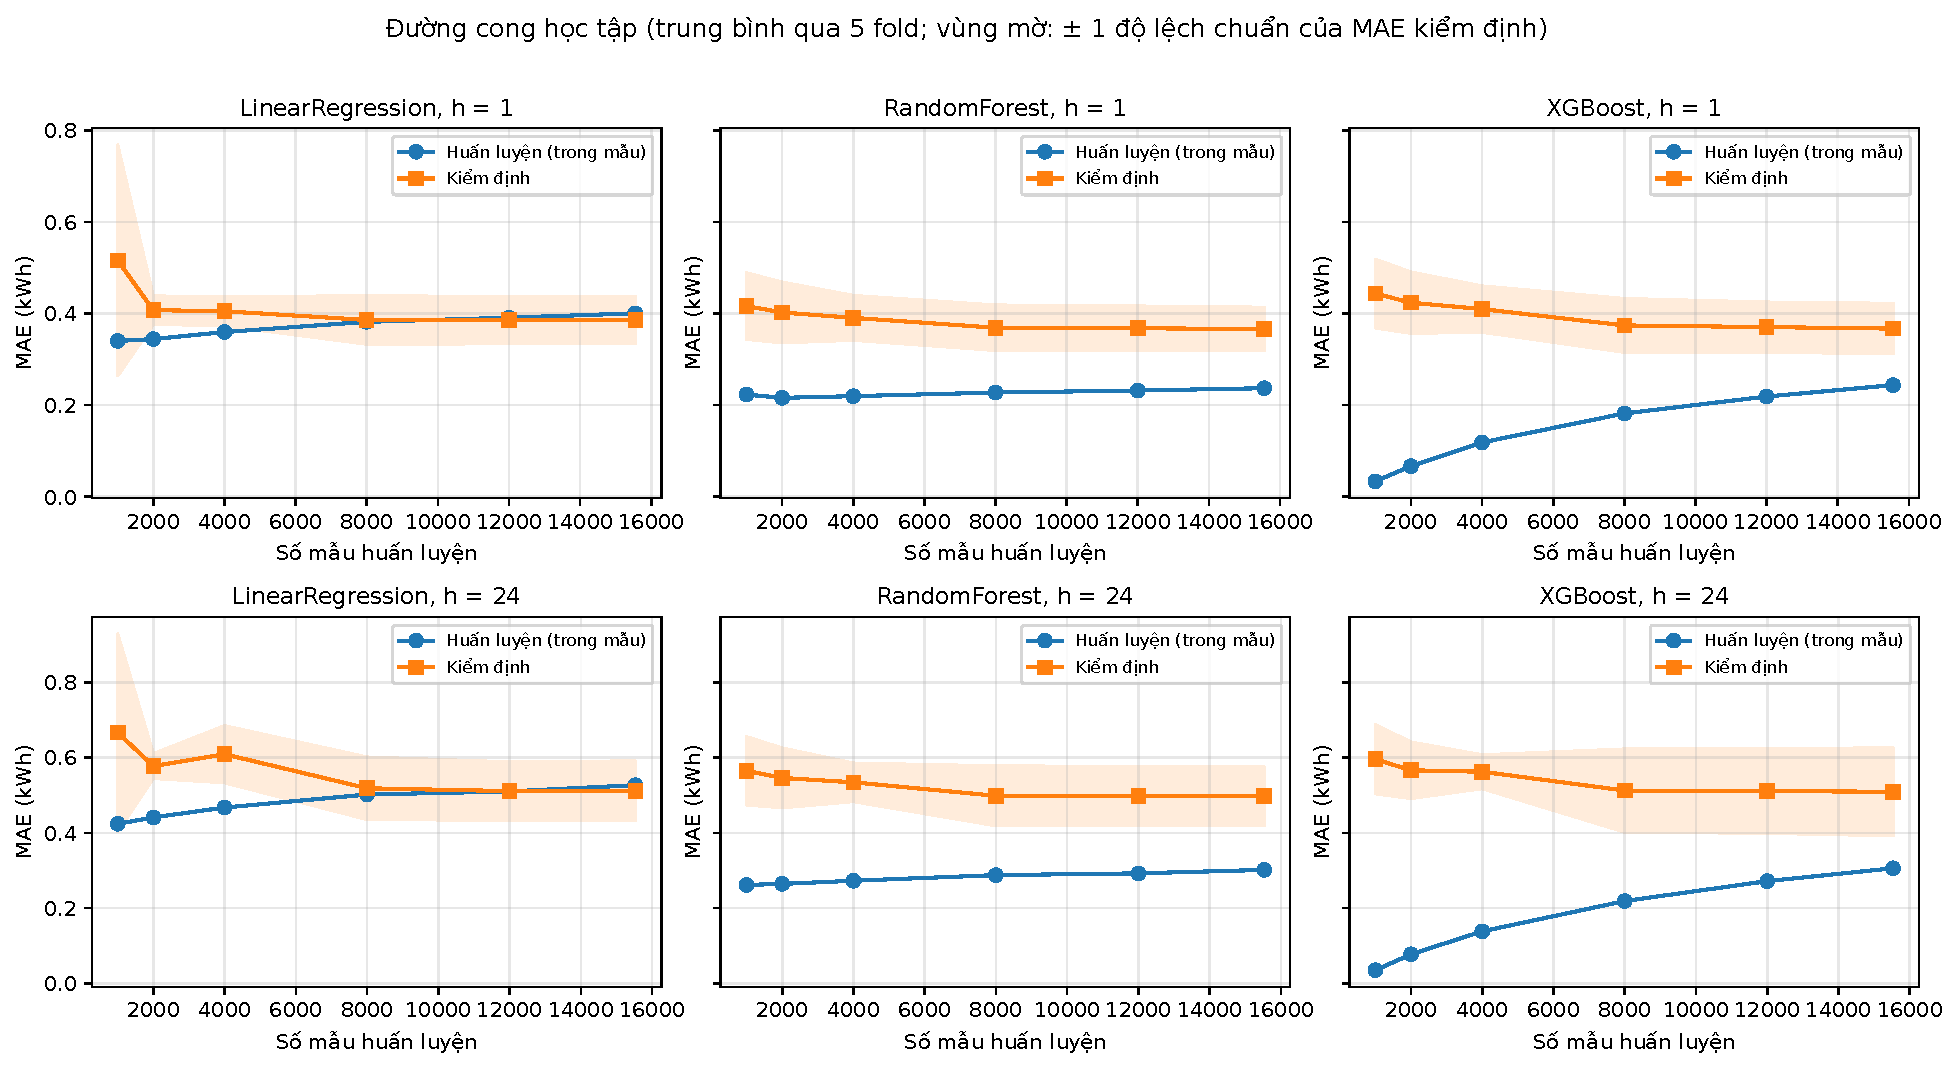
\includegraphics[width=\textwidth]{figures/duong_cong_hoc_tap.pdf}
    \caption{Đường cong học tập (trung bình qua 5 fold; vùng mờ: $\pm$ một độ lệch chuẩn của MAE kiểm định).}
    \label{fig:learning_curve}
\end{figure}

\subsection{Đường cong kiểm định}
Để kiểm chứng dấu hiệu quá khớp nêu ở Mục~\ref{sec:train_val}, nhóm thay đổi siêu tham số điều khiển độ phức tạp của từng mô hình cây (số mẫu tối thiểu ở lá của Random Forest từ 1 đến 200; độ sâu tối đa của XGBoost từ 2 đến 10), mỗi giá trị chạy đủ 5 fold (Hình~\ref{fig:validation_curve}). Khi độ phức tạp tăng, sai số trong mẫu giảm rất mạnh (Random Forest từ 0,405 xuống 0,142 kWh, XGBoost từ 0,386 xuống 0,077 kWh ở $h = 1$), nhưng sai số kiểm định gần như không đổi: Random Forest đạt 0,365--0,372 kWh với số mẫu ở lá từ 1 đến 50 (thấp nhất ở 5--10) và chỉ tăng rõ khi cây quá đơn giản (0,390 kWh với 200 mẫu); XGBoost đạt 0,364--0,376 kWh với độ sâu từ 2 đến 10 (thấp nhất ở độ sâu 4). Ở $h = 24$ đường kiểm định còn phẳng hơn.

Như vậy khoảng cách giữa sai số trong mẫu và sai số kiểm định ở Chương~\ref{chap:models} chủ yếu do cách đo trong mẫu của mô hình cây, không phải quá khớp gây hại: giảm độ phức tạp không làm sai số kiểm định giảm, và cấu hình ban đầu đã nằm gần đáy của đường kiểm định. Do đó cải tiến cần đến từ thông tin mới (đặc trưng) hơn là từ điều chuẩn mạnh hơn.

\begin{figure}[htbp]
    \centering
    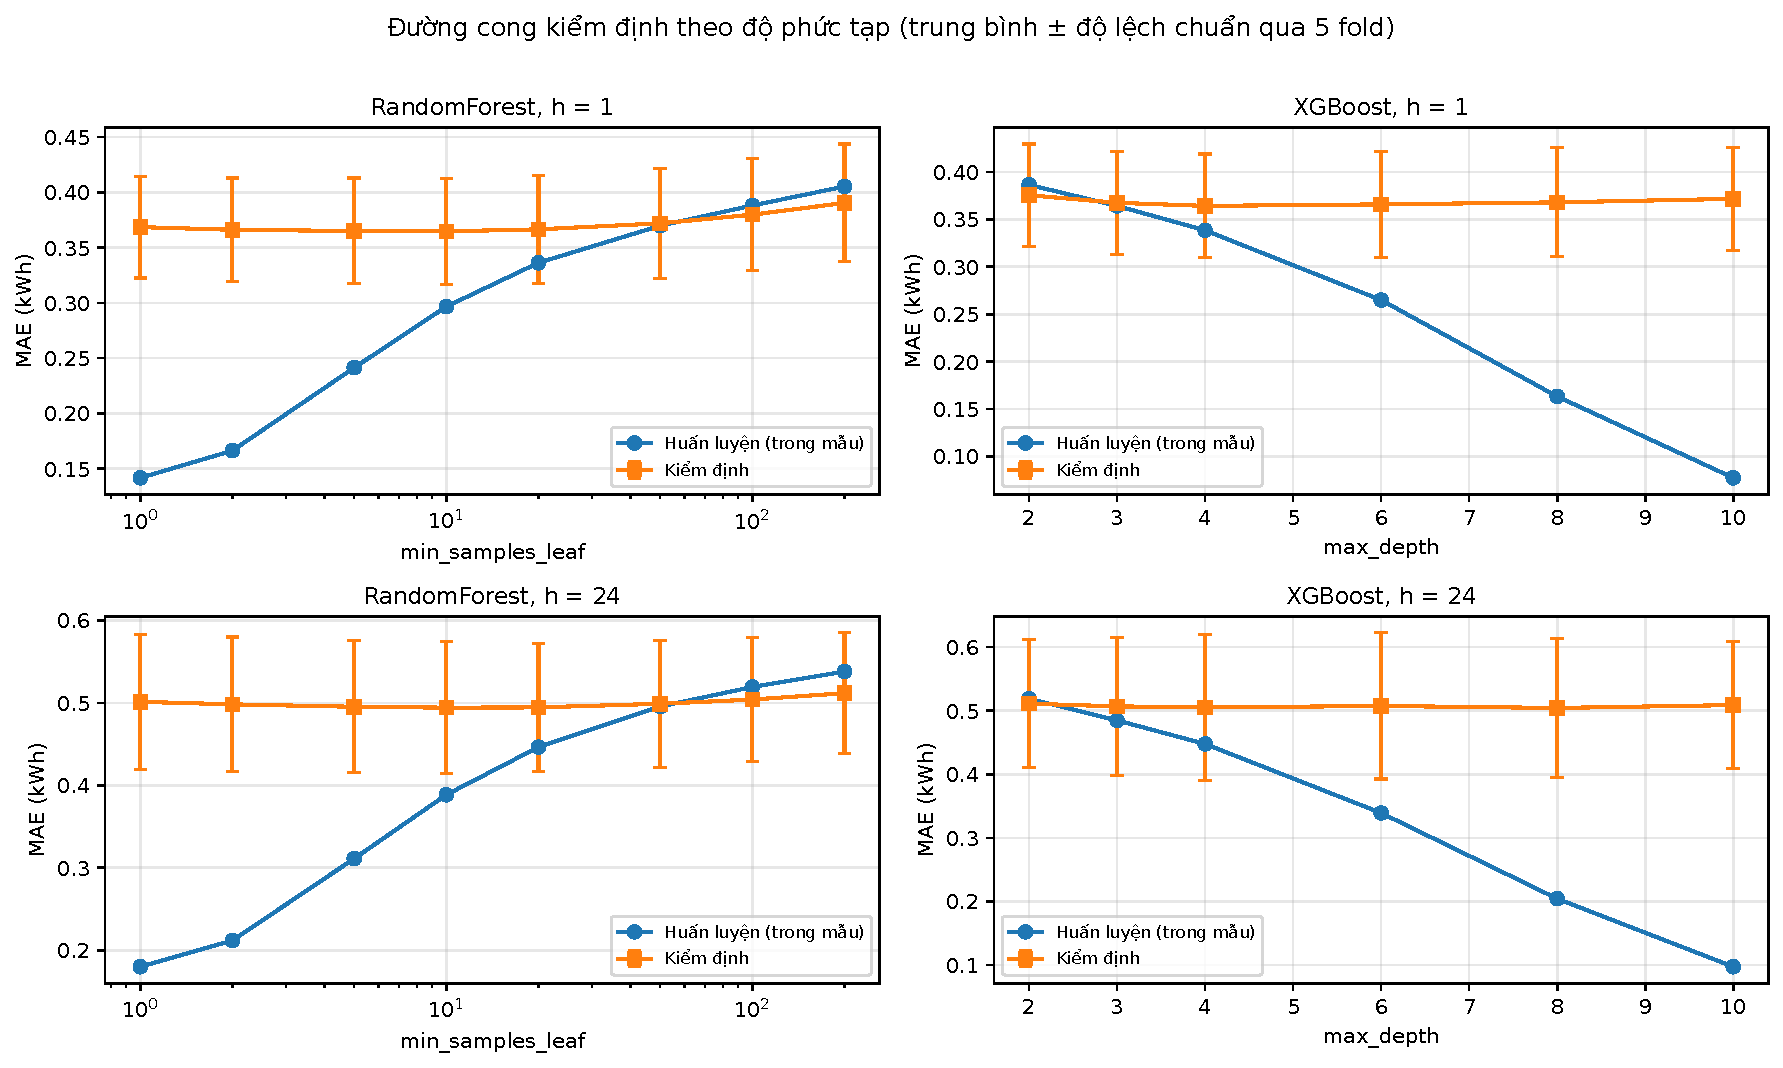
\includegraphics[width=\textwidth]{figures/duong_cong_kiem_dinh.pdf}
    \caption{Đường cong kiểm định theo độ phức tạp của mô hình cây (trung bình $\pm$ độ lệch chuẩn qua 5 fold).}
    \label{fig:validation_curve}
\end{figure}

\subsection{Hạn chế và giải pháp đề xuất}
Kết hợp hai đường cong trên với phân tích lỗi ở Mục~\ref{sec:error_analysis}, nhóm tổng hợp các hạn chế và giải pháp tương ứng ở Bảng~\ref{tab:limits}.

\begin{table}[htbp]
    \centering
    \caption{Hạn chế của mô hình ban đầu và giải pháp đề xuất.}
    \label{tab:limits}
    \small
    \begin{tabularx}{\textwidth}{|>{\raggedright\arraybackslash}p{3.6cm}|>{\raggedright\arraybackslash}X|>{\raggedright\arraybackslash}p{4.2cm}|}
        \hline
        \textbf{Hạn chế} & \textbf{Bằng chứng} & \textbf{Giải pháp và cơ sở} \\ \hline
        Không biết thiết bị nào đang chạy, dự báo thấp các giờ đỉnh & 5\% giờ cao nhất bị dự báo thấp 1,06--1,63 kWh (Bảng~\ref{tab:error_conc}); ở $h = 1$, điện năng giờ vừa qua áp đảo tầm quan trọng (Hình~\ref{fig:importance}) & Thêm điện năng của ba nhóm công tơ phụ tại $t$ và $t-1$: thông tin quá khứ của chuỗi liên quan, có sẵn tại $t$ \\ \hline
        Đặc trưng lịch không phân biệt ngày lễ với ngày thường & Đặc trưng thứ trong tuần coi ngày lễ giữa tuần như ngày làm việc & Cờ ngày lễ Pháp và ngày liền kề: biến biết trước về thời điểm mục tiêu \\ \hline
        Siêu tham số chọn theo giá trị phổ biến & Chưa được kiểm chứng ở Chương~\ref{chap:models} & Tìm kiếm ngẫu nhiên trên cùng 5 fold kiểm định chéo \\ \hline
        Linear Regression chưa khớp & Hai đường cong học tập gặp nhau ở mức sai số cao (Hình~\ref{fig:learning_curve}) & Thử Ridge để kiểm tra; dự kiến điều chuẩn không giúp vì vấn đề là độ chệch \\ \hline
        Random Forest và XGBoost có sai số gần nhau nhưng xây dựng khác nhau & Chênh lệch MAE không quá 0,013 kWh (Bảng~\ref{tab:cv_summary}) & Tổ hợp Voting lấy trung bình hai mô hình \\ \hline
        Thêm dữ liệu cùng loại gần như không giúp & Sai số kiểm định đi ngang từ khoảng 8.000 mẫu (Hình~\ref{fig:learning_curve}) & Ưu tiên thêm thông tin mới (đặc trưng) thay vì thêm mẫu \\ \hline
    \end{tabularx}
\end{table}

Quá khớp của mô hình cây không được đưa vào bảng vì đường cong kiểm định không xác nhận nó.

\section{Cải tiến đặc trưng}
\label{sec:feat_improve}

Hai nhóm đặc trưng mới được thêm vào bộ 21 đặc trưng ban đầu:
\begin{itemize}
    \item Điện năng của từng nhóm công tơ phụ (bếp; giặt là; bình nước nóng và điều hòa) tại $t$ và $t-1$, gồm 6 đặc trưng. Phần điện năng còn lại không được thêm vì nó bằng điện năng tổng trừ ba công tơ phụ, nên đã nằm trong các đặc trưng hiện có. Các giá trị này chỉ dùng dữ liệu đến thời điểm gốc $t$.
    \item Cờ ngày lễ Pháp của ngày mục tiêu và cờ ngày liền kề ngày lễ (trước hoặc sau một ngày), gồm 2 đặc trưng, lấy từ thư viện holidays. Lịch ngày lễ biết trước nên dùng được cho thời điểm mục tiêu.
\end{itemize}
Notebook kiểm tra lại rằng các đặc trưng mới không dùng thông tin tương lai bằng cùng phép thử như Mục~\ref{sec:features}. Để tách riêng tác động của dữ liệu, siêu tham số được giữ như Chương~\ref{chap:models}, chỉ đổi bộ đặc trưng (Bảng~\ref{tab:feat_delta}, Hình~\ref{fig:feat}).

\begin{table}[htbp]
\centering
\caption[Tác động của đặc trưng mới]{Thay đổi MAE kiểm định chéo (\%) khi thêm đặc trưng mới so với bộ 21 đặc trưng ban đầu, siêu tham số giữ nguyên; trong ngoặc là số fold có MAE thấp hơn. Giá trị âm là tốt hơn.}
\label{tab:feat_delta}
\small
\begin{tabular}{|l|l|c|c|c|c|}
\hline
\textbf{Mô hình} & \textbf{Đặc trưng thêm} & \textbf{$h = 1$} & \textbf{$h = 6$} & \textbf{$h = 12$} & \textbf{$h = 24$} \\
\hline
\multirow{3}{*}{Linear Regression} & Công tơ phụ & $-$1{,}5 (5/5) & $-$0{,}5 (4/5) & $-$1{,}0 (5/5) & $-$0{,}6 (5/5) \\
\cline{2-6}
 & Ngày lễ & 0{,}0 (1/5) & 0{,}0 (3/5) & 0{,}0 (3/5) & 0{,}0 (2/5) \\
\cline{2-6}
 & Cả hai & $-$1{,}5 (5/5) & $-$0{,}4 (4/5) & $-$1{,}0 (5/5) & $-$0{,}6 (5/5) \\
\hline
\multirow{3}{*}{Random Forest} & Công tơ phụ & $-$3{,}8 (5/5) & 0{,}0 (2/5) & 0{,}1 (3/5) & 0{,}1 (2/5) \\
\cline{2-6}
 & Ngày lễ & $-$0{,}2 (3/5) & $-$0{,}1 (2/5) & 0{,}1 (1/5) & $-$0{,}1 (3/5) \\
\cline{2-6}
 & Cả hai & $-$3{,}8 (5/5) & $-$0{,}1 (2/5) & 0{,}1 (3/5) & 0{,}1 (2/5) \\
\hline
\multirow{3}{*}{XGBoost} & Công tơ phụ & $-$8{,}0 (5/5) & $-$1{,}6 (3/5) & $-$0{,}8 (3/5) & $-$0{,}3 (4/5) \\
\cline{2-6}
 & Ngày lễ & 0{,}6 (2/5) & $-$0{,}9 (3/5) & 0{,}0 (2/5) & $-$0{,}7 (4/5) \\
\cline{2-6}
 & Cả hai & $-$8{,}3 (5/5) & $-$0{,}9 (2/5) & $-$0{,}7 (3/5) & $-$0{,}3 (3/5) \\
\hline
\end{tabular}
\end{table}


\begin{figure}[htbp]
    \centering
    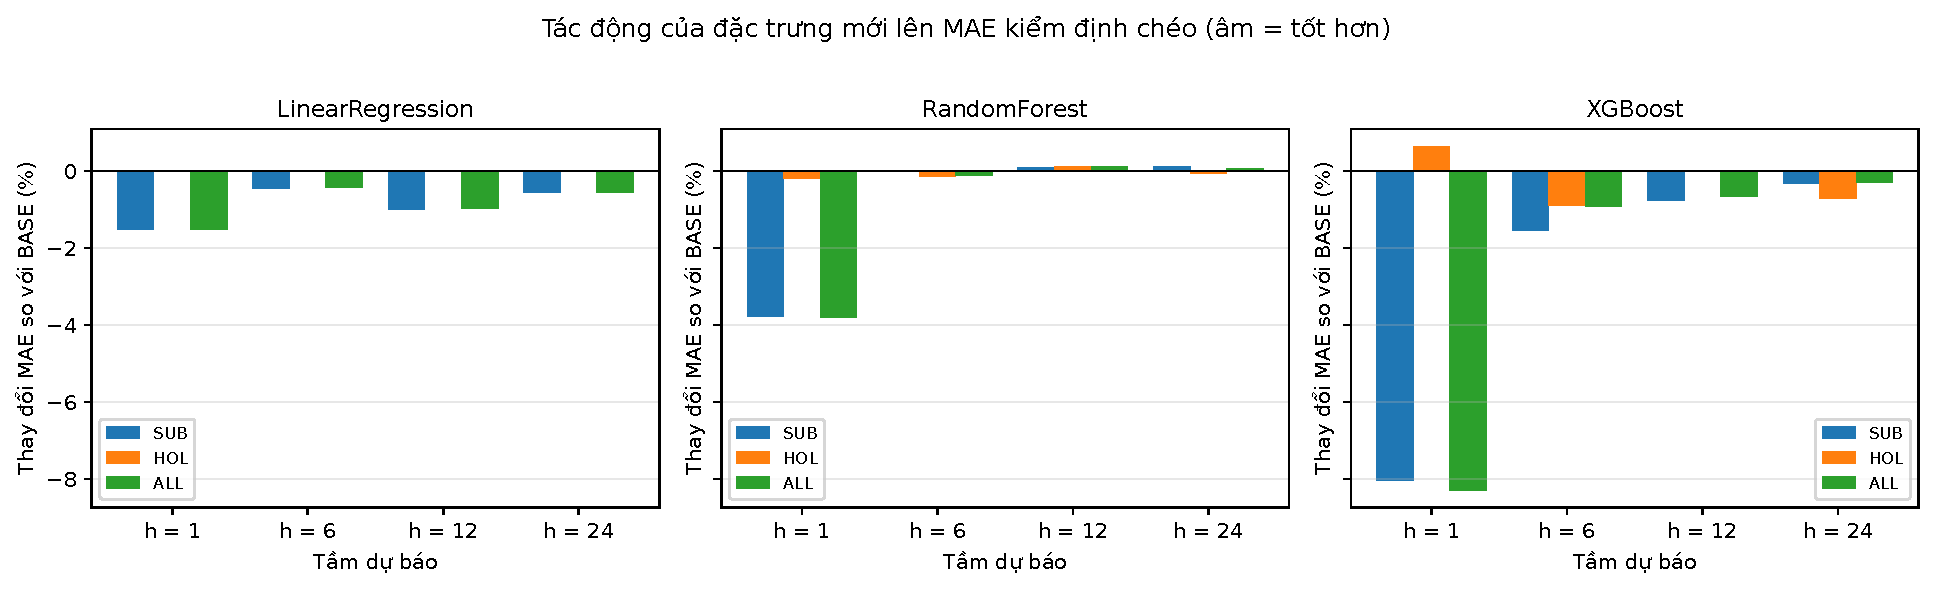
\includegraphics[width=\textwidth]{figures/cai_tien_dac_trung.pdf}
    \caption{Thay đổi MAE kiểm định chéo khi thêm đặc trưng mới so với bộ đặc trưng ban đầu (âm là tốt hơn).}
    \label{fig:feat}
\end{figure}

Đặc trưng công tơ phụ giúp rõ ở $h = 1$: XGBoost giảm MAE 8,0\% (0,366 xuống 0,336 kWh), Random Forest 3,8\%, Linear Regression 1,5\%, và cả ba mô hình đều tốt hơn ở 5/5 fold. Một chu trình giặt hay đun nước thường kéo dài quá một giờ, nên biết thiết bị nào đang chạy giúp đoán giờ kế tiếp. Ở $h \ge 6$, tác động nhỏ (từ $-1{,}6\%$ đến $+0{,}1\%$); Linear Regression vẫn cải thiện nhẹ ở 4--5/5 fold, còn với hai mô hình cây kết quả không nhất quán qua các fold (2--4/5), vì trạng thái thiết bị cách sáu giờ trở lên không còn liên quan đến giờ mục tiêu.

Đặc trưng ngày lễ gần như không có tác động (từ $-0{,}9\%$ đến $+0{,}6\%$, số fold cải thiện không có xu hướng). Tập huấn luyện chỉ có 768 giờ ngày lễ (32 ngày), quá ít để mô hình học được một mẫu tiêu thụ riêng, và hộ này có thể không thay đổi thói quen nhiều vào ngày lễ. Đây là một cải tiến không thành công nhưng vẫn cho biết thêm về dữ liệu.

Bộ đặc trưng dùng cho các bước sau được chọn theo quy tắc định trước: bộ có MAE trung bình thấp nhất khi lấy trung bình qua ba mô hình và bốn tầm dự báo. Bộ có công tơ phụ (27 đặc trưng) được chọn (MAE trung bình 0,4598 kWh, so với 0,4600 khi thêm cả ngày lễ và 0,4658 với bộ ban đầu).

\section{Tối ưu siêu tham số}
\label{sec:tuning}

Siêu tham số của Random Forest và XGBoost được tìm bằng tìm kiếm ngẫu nhiên (lần lượt 20 và 30 cấu hình), của Ridge bằng tìm kiếm lưới trên 11 giá trị $\alpha$ từ $0{,}01$ đến $1000$ (thang logarit), theo~\eqref{eq:hpo} với $K = 5$ và chỉ số MAE. Tìm kiếm dùng chính 5 fold thời gian ở các mục trước, phần kiểm định đã lọc về tập mẫu dùng chung, nên điểm tìm kiếm trùng với điểm của quy trình kiểm định chéo. Không gian tìm kiếm được đặt quanh các giá trị phổ biến:
\begin{itemize}
    \item Random Forest (300 cây): số mẫu tối thiểu ở lá $\{1, 2, 5, 10, 20, 50\}$; tỷ lệ đặc trưng mỗi lần tách $\{0{,}2; 0{,}33; 0{,}5; 0{,}7; 1\}$; độ sâu tối đa $\{12, 20, \text{không giới hạn}\}$.
    \item XGBoost: số cây $\{200, 400, 800\}$; tốc độ học $\{0{,}01; 0{,}03; 0{,}05; 0{,}1\}$; độ sâu tối đa $\{3, 4, 5, 6, 8\}$; tổng trọng số tối thiểu ở lá $\{1, 5, 10, 20\}$; tỷ lệ mẫu mỗi cây $\{0{,}6; 0{,}8; 1\}$; tỷ lệ đặc trưng mỗi cây $\{0{,}5; 0{,}7; 0{,}9; 1\}$; hệ số phạt L2 $\{0{,}1; 1; 10\}$.
\end{itemize}
Toàn bộ tìm kiếm cho bốn tầm dự báo chạy khoảng 30 phút trên máy 16 luồng. Bảng~\ref{tab:best_params} liệt kê cấu hình tốt nhất.

\begin{table}[htbp]
\centering
\caption[Siêu tham số tối ưu]{Siêu tham số tốt nhất tìm được bằng tìm kiếm trên 5 fold kiểm định chéo.}
\label{tab:best_params}
\footnotesize\setlength{\tabcolsep}{4pt}
\begin{tabular}{|l|l|c|c|c|c|}
\hline
\textbf{Mô hình} & \textbf{Siêu tham số} & \textbf{$h = 1$} & \textbf{$h = 6$} & \textbf{$h = 12$} & \textbf{$h = 24$} \\
\hline
\multirow{3}{*}{Random Forest} & Số mẫu tối thiểu ở lá & 5 & 10 & 10 & 20 \\
\cline{2-6}
 & Tỷ lệ đặc trưng mỗi lần tách & 1{,}00 & 0{,}70 & 0{,}70 & 0{,}70 \\
\cline{2-6}
 & Độ sâu tối đa & không giới hạn & 20 & 20 & không giới hạn \\
\hline
\multirow{7}{*}{XGBoost} & Số cây & 400 & 200 & 800 & 200 \\
\cline{2-6}
 & Tốc độ học & 0{,}03 & 0{,}03 & 0{,}01 & 0{,}03 \\
\cline{2-6}
 & Độ sâu tối đa & 8 & 6 & 6 & 6 \\
\cline{2-6}
 & Tổng trọng số tối thiểu ở lá & 20 & 1 & 10 & 1 \\
\cline{2-6}
 & Tỷ lệ mẫu mỗi cây & 1{,}00 & 0{,}80 & 1{,}00 & 0{,}80 \\
\cline{2-6}
 & Tỷ lệ đặc trưng mỗi cây & 0{,}90 & 0{,}90 & 0{,}70 & 0{,}90 \\
\cline{2-6}
 & Hệ số phạt L2 ($\lambda$) & 10 & 10 & 0{,}10 & 10 \\
\hline
\multirow{1}{*}{Ridge} & $\alpha$ & 10 & 0{,}01 & 0{,}01 & 0{,}01 \\
\hline
\end{tabular}
\end{table}


\begin{figure}[htbp]
    \centering
    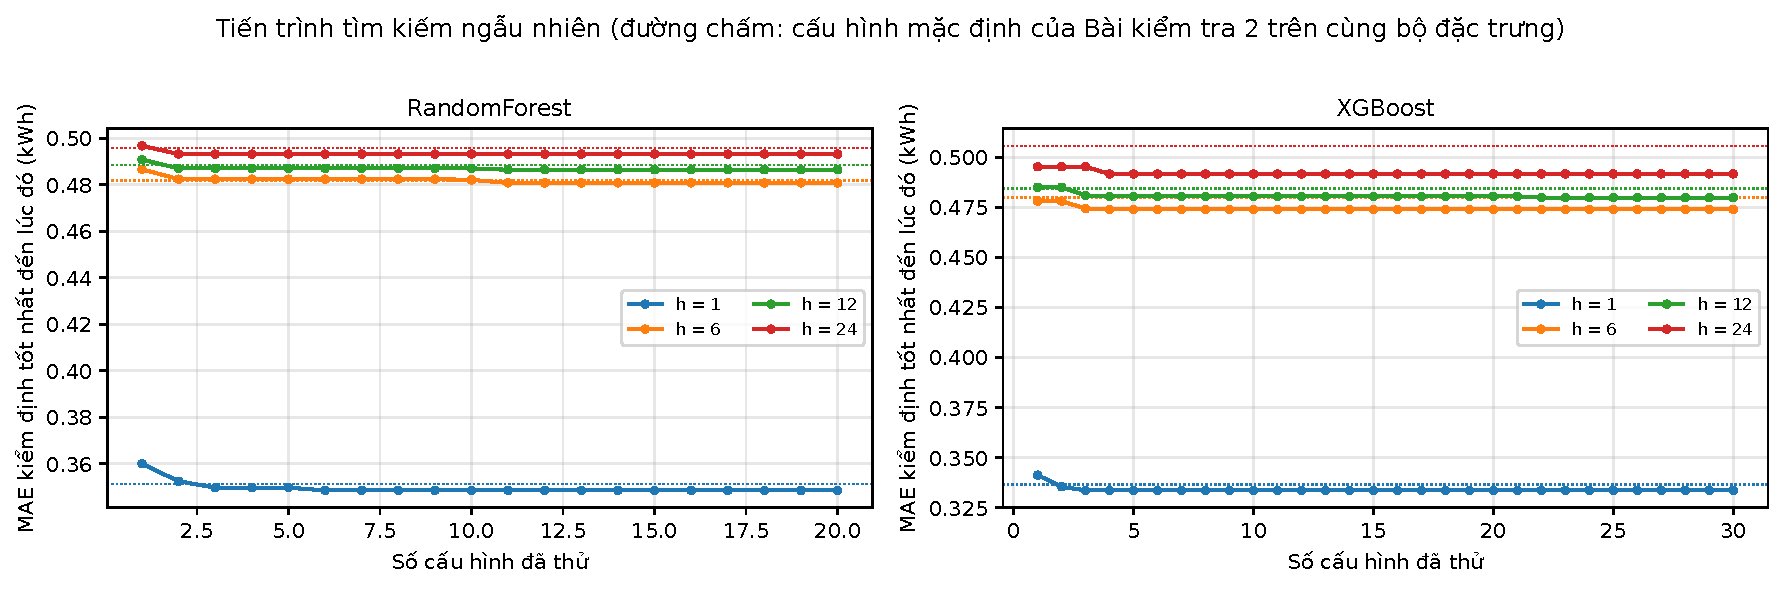
\includegraphics[width=\textwidth]{figures/tim_kiem.pdf}
    \caption{MAE kiểm định tốt nhất đạt được theo số cấu hình đã thử (đường chấm: cấu hình ban đầu trên cùng bộ đặc trưng).}
    \label{fig:search}
\end{figure}

Mức cải thiện so với cấu hình ban đầu trên cùng bộ đặc trưng là nhỏ: Random Forest giảm 0,001--0,003 kWh, XGBoost giảm 0,003 kWh ($h = 1$) đến 0,014 kWh ($h = 24$, từ 0,506 xuống 0,492 kWh), đều nhỏ hơn độ lệch chuẩn giữa các fold (0,05--0,11 kWh). Hình~\ref{fig:search} cho thấy phần lớn mức cải thiện đạt được trong khoảng năm lần thử đầu; các cấu hình tìm thấy muộn hơn chỉ tốt hơn thêm dưới 0,002 kWh, nên mở rộng ngân sách tìm kiếm khó cải thiện đáng kể. Điều này khớp với đường cong kiểm định phẳng ở Hình~\ref{fig:validation_curve}. Ridge chọn $\alpha$ ở đầu dưới của lưới ($0{,}01$ với $h \ge 6$; ở $h = 1$, $\alpha = 10$ nhưng MAE chỉ khác Linear Regression 0,0003 kWh), xác nhận rằng điều chuẩn không giúp mô hình tuyến tính vốn chưa khớp. Một số giá trị tối ưu nằm ở biên không gian tìm kiếm (XGBoost độ sâu 8 và Random Forest xét toàn bộ đặc trưng ở $h = 1$); vì chênh lệch giữa các cấu hình tốt rất nhỏ, nhóm không mở rộng thêm không gian.

Cần lưu ý rằng điểm kiểm định chéo của cấu hình được chọn hơi lạc quan, vì chính các fold này được dùng để chọn nó~\cite{bischl2023hyperparameter}. Ước lượng không bị ảnh hưởng bởi lựa chọn là kết quả trên tập kiểm tra ở Mục~\ref{sec:test}.

\section{So sánh trước và sau cải tiến}
\label{sec:ablation}

Ngoài các mô hình ở Chương~\ref{chap:models}, nhóm thử hai mô hình mới: Ridge~\eqref{eq:ridge}, cùng tiền xử lý với Linear Regression, và tổ hợp Voting~\eqref{eq:voting} lấy trung bình dự báo của Random Forest và XGBoost đã tối ưu. Bảng~\ref{tab:ablation} và Hình~\ref{fig:ablation} trình bày kết quả qua từng bước cải tiến, mỗi bước chỉ thay đổi một yếu tố so với bước trước.

\begin{table}[htbp]
\centering
\caption[So sánh trước và sau cải tiến (ablation)]{MAE kiểm định chéo (kWh, trung bình $\pm$ độ lệch chuẩn qua 5 fold) qua từng bước cải tiến, cùng dữ liệu, cùng 5 fold và cùng tập mẫu. A0: cấu hình Bài kiểm tra 2; A1: thêm đặc trưng công tơ phụ; A2: tối ưu siêu tham số; A3: tổ hợp Voting.}
\label{tab:ablation}
\footnotesize\setlength{\tabcolsep}{4pt}
\begin{tabular}{|c|l|c|c|c|c|}
\hline
\textbf{Bước} & \textbf{Mô hình} & \textbf{$h = 1$} & \textbf{$h = 6$} & \textbf{$h = 12$} & \textbf{$h = 24$} \\
\hline
\multirow{2}{*}{Cơ sở} & Naive & 0{,}440 $\pm$ 0{,}069 & 0{,}971 $\pm$ 0{,}186 & 0{,}781 $\pm$ 0{,}207 & 0{,}630 $\pm$ 0{,}128 \\
\cline{2-6}
 & SNaive168 & 0{,}602 $\pm$ 0{,}127 & 0{,}602 $\pm$ 0{,}127 & 0{,}602 $\pm$ 0{,}127 & 0{,}603 $\pm$ 0{,}127 \\
\hline
\multirow{3}{*}{A0} & Linear Regression & 0{,}384 $\pm$ 0{,}052 & 0{,}508 $\pm$ 0{,}081 & 0{,}509 $\pm$ 0{,}083 & 0{,}507 $\pm$ 0{,}088 \\
\cline{2-6}
 & Random Forest & 0{,}365 $\pm$ 0{,}048 & 0{,}482 $\pm$ 0{,}078 & 0{,}488 $\pm$ 0{,}078 & 0{,}495 $\pm$ 0{,}080 \\
\cline{2-6}
 & XGBoost & 0{,}366 $\pm$ 0{,}056 & 0{,}488 $\pm$ 0{,}107 & 0{,}488 $\pm$ 0{,}096 & 0{,}507 $\pm$ 0{,}115 \\
\hline
\multirow{3}{*}{A1} & Linear Regression & 0{,}378 $\pm$ 0{,}049 & 0{,}506 $\pm$ 0{,}081 & 0{,}504 $\pm$ 0{,}083 & 0{,}505 $\pm$ 0{,}086 \\
\cline{2-6}
 & Random Forest & 0{,}351 $\pm$ 0{,}046 & 0{,}482 $\pm$ 0{,}077 & 0{,}488 $\pm$ 0{,}077 & 0{,}496 $\pm$ 0{,}078 \\
\cline{2-6}
 & XGBoost & 0{,}336 $\pm$ 0{,}050 & 0{,}480 $\pm$ 0{,}091 & 0{,}485 $\pm$ 0{,}092 & 0{,}506 $\pm$ 0{,}114 \\
\hline
\multirow{3}{*}{A2} & Ridge & 0{,}378 $\pm$ 0{,}050 & 0{,}506 $\pm$ 0{,}081 & 0{,}504 $\pm$ 0{,}083 & 0{,}505 $\pm$ 0{,}086 \\
\cline{2-6}
 & Random Forest & 0{,}348 $\pm$ 0{,}046 & 0{,}481 $\pm$ 0{,}078 & 0{,}486 $\pm$ 0{,}078 & 0{,}493 $\pm$ 0{,}079 \\
\cline{2-6}
 & XGBoost & 0{,}334 $\pm$ 0{,}050 & 0{,}474 $\pm$ 0{,}084 & 0{,}480 $\pm$ 0{,}085 & 0{,}492 $\pm$ 0{,}098 \\
\hline
\multirow{1}{*}{A3} & Voting (RF + XGBoost) & 0{,}337 $\pm$ 0{,}047 & 0{,}476 $\pm$ 0{,}081 & 0{,}481 $\pm$ 0{,}082 & 0{,}491 $\pm$ 0{,}088 \\
\hline
\end{tabular}
\end{table}


\begin{figure}[htbp]
    \centering
    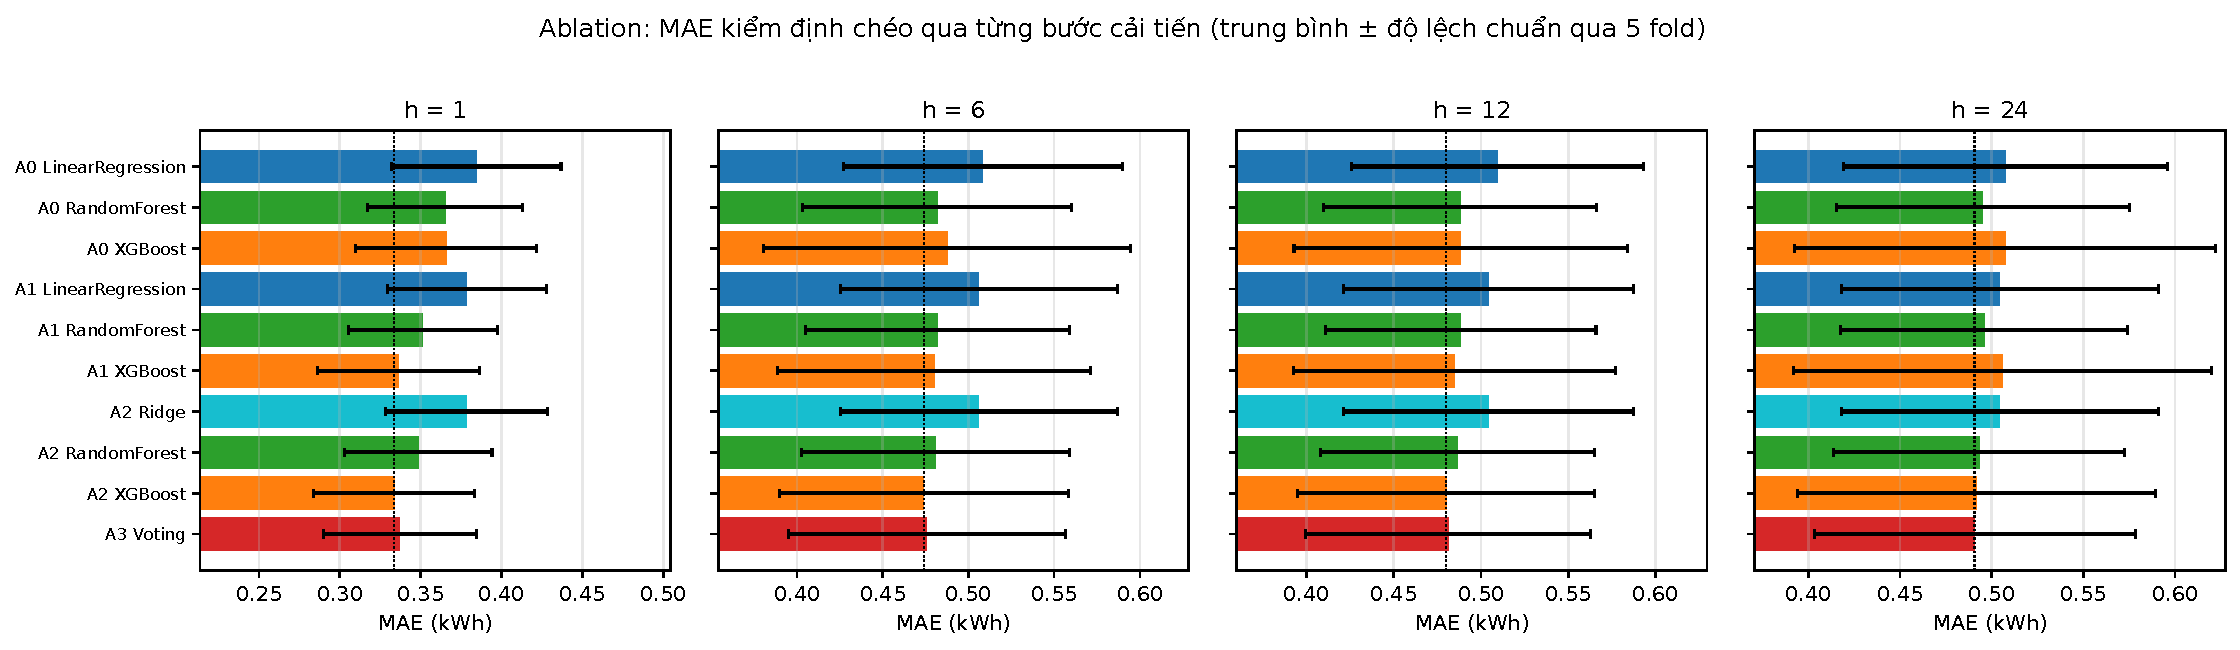
\includegraphics[width=\textwidth]{figures/ablation.pdf}
    \caption{MAE kiểm định chéo qua từng bước cải tiến (trung bình $\pm$ độ lệch chuẩn qua 5 fold; đường chấm: giá trị thấp nhất).}
    \label{fig:ablation}
\end{figure}

\begin{itemize}
    \item Ở $h = 1$, cải tiến lớn nhất đến từ đặc trưng công tơ phụ. MAE tốt nhất giảm từ 0,365 (Random Forest, A0) xuống 0,334 kWh (XGBoost, A2), tức 8,6\%; với XGBoost, bước thêm đặc trưng đóng góp 0,029 kWh, bước tối ưu thêm 0,003 kWh. XGBoost A2 tốt hơn XGBoost A0 ở cả 5/5 fold.
    \item Ở $h \ge 6$, cải tiến nhỏ: MAE tốt nhất giảm 1,6\% ở $h = 6$ và $h = 12$ (nhờ XGBoost đã tối ưu) và 0,9\% ở $h = 24$ (Voting; riêng XGBoost đã tối ưu giảm 0,7\%). Các mức này nhỏ hơn độ lệch chuẩn giữa các fold, nhưng XGBoost A2 tốt hơn XGBoost A0 ở 3--5/5 fold.
    \item Ridge cho MAE trùng Linear Regression cùng bộ đặc trưng đến bốn chữ số thập phân ở $h \ge 6$, xác nhận mô hình tuyến tính bị giới hạn bởi độ chệch.
    \item Voting không tốt hơn mô hình đơn tốt nhất một cách có ý nghĩa. Ở $h = 1$, Voting kém XGBoost (0,337 so với 0,334 kWh) vì Random Forest yếu hơn rõ rệt và kéo trung bình lên; ở $h = 24$, Voting tốt hơn XGBoost chỉ 0,001 kWh. Một giải thích có thể là hai mô hình cây học cùng các quan hệ từ cùng đặc trưng nên sai số của chúng giống nhau ở nhiều giờ, khiến lấy trung bình không giảm được bao nhiêu; nhóm chưa đo trực tiếp mức tương quan này.
\end{itemize}

\section{Lựa chọn mô hình cuối}
\label{sec:final_model}

Mô hình cuối được chọn theo quy tắc định trước, chỉ dùng kết quả kiểm định chéo: trong các mô hình ở bước A2 và A3, chọn mô hình có MAE trung bình thấp nhất ở mỗi tầm dự báo; nếu Voting chỉ tốt hơn mô hình đơn tốt nhất dưới 1\% thì chọn mô hình đơn đó, vì tổ hợp tốn thời gian huấn luyện gấp nhiều lần và khó diễn giải hơn mà lợi ích không đáng kể so với độ lệch giữa các fold.

Theo quy tắc này, XGBoost đã tối ưu với 27 đặc trưng được chọn ở cả bốn tầm dự báo (MAE kiểm định chéo 0,334; 0,474; 0,480 và 0,492 kWh). Các yếu tố đánh đổi khác:
\begin{itemize}
    \item Thời gian: XGBoost huấn luyện nhanh nhất trong các mô hình cây (dưới 2 giây mỗi fold trên máy 16 luồng, so với khoảng 3--6 giây của Random Forest và 4--7 giây của Voting; thời gian thay đổi nhẹ giữa các lần chạy).
    \item Độ ổn định: độ lệch chuẩn qua các fold của XGBoost ở $h \ge 6$ (0,084--0,098 kWh) lớn hơn Random Forest (0,078--0,079 kWh), tức XGBoost kém ổn định hơn một chút giữa các mùa.
    \item Khả năng diễn giải: hai mô hình cây tương đương, đều cần tầm quan trọng hoán vị để giải thích; Ridge dễ diễn giải nhất nhưng MAE cao hơn XGBoost 0,013--0,045 kWh.
\end{itemize}
Cấu hình cuối được ghi ra file trước khi dùng tập kiểm tra.

\section{Đánh giá trên tập kiểm tra}
\label{sec:test}

Mỗi mô hình được huấn luyện lại trên toàn bộ tập huấn luyện (nhãn đến 31/12/2009) với cấu hình đã chốt, rồi dự báo các giờ của năm 2010 (01/01--26/11/2010; 7.227 giờ thuộc tập mẫu dùng chung cho mỗi tầm dự báo). Tập kiểm tra chỉ được dùng ở mục này, sau khi mọi lựa chọn đã được chốt, và kết quả chỉ dùng để báo cáo. Để thấy tác động của toàn bộ quá trình cải tiến, Bảng~\ref{tab:test} gồm cả mô hình cơ sở và mô hình của Chương~\ref{chap:models}.

\begin{table}[htbp]
\centering
\caption[Kết quả trên tập kiểm tra]{MAE (kWh) trên tập kiểm tra năm 2010 (7.227 giờ cho mỗi tầm dự báo). Mô hình được huấn luyện lại trên toàn bộ tập huấn luyện với cấu hình đã chốt.}
\label{tab:test}
\small
\begin{tabular}{|l|c|c|c|c|}
\hline
\textbf{Mô hình} & \textbf{$h = 1$} & \textbf{$h = 6$} & \textbf{$h = 12$} & \textbf{$h = 24$} \\
\hline
Mean & 0{,}650 & 0{,}650 & 0{,}650 & 0{,}650 \\ \hline
Naive & 0{,}408 & 0{,}854 & 0{,}715 & 0{,}556 \\ \hline
SNaive24 & 0{,}556 & 0{,}556 & 0{,}556 & 0{,}556 \\ \hline
SNaive168 & 0{,}577 & 0{,}577 & 0{,}577 & 0{,}577 \\ \hline
Linear Regression (A0) & 0{,}361 & 0{,}470 & 0{,}469 & 0{,}465 \\ \hline
Random Forest (A0) & 0{,}336 & 0{,}438 & 0{,}444 & 0{,}448 \\ \hline
XGBoost (A0) & 0{,}334 & 0{,}440 & 0{,}449 & 0{,}445 \\ \hline
Ridge (A2) & 0{,}359 & 0{,}468 & 0{,}466 & 0{,}463 \\ \hline
Random Forest (A2) & 0{,}322 & 0{,}438 & 0{,}443 & 0{,}446 \\ \hline
XGBoost (A2, mô hình cuối) & 0{,}313 & 0{,}434 & 0{,}439 & 0{,}441 \\ \hline
Voting (A3) & 0{,}314 & 0{,}435 & 0{,}439 & 0{,}442 \\ \hline
\end{tabular}
\end{table}


\begin{table}[htbp]
\centering
\caption[Kiểm định chéo và tập kiểm tra của mô hình cuối]{Mô hình cuối (XGBoost đã tối ưu): MAE kiểm định chéo so với kết quả trên tập kiểm tra, và mức giảm MAE so với mô hình cơ sở được chọn trên kiểm định chéo (MAE của mô hình cơ sở đó trên tập kiểm tra trong ngoặc).}
\label{tab:cv_test}
\footnotesize\setlength{\tabcolsep}{4pt}
\begin{tabular}{|c|c|c|c|c|c|c|}
\hline
\textbf{$h$} & \textbf{MAE KĐC} & \textbf{MAE KT} & \textbf{RMSE KT} & \textbf{MAPE KT (\%)} & \textbf{Cơ sở (MAE KT)} & \textbf{Giảm (\%)} \\
\hline
1 & 0{,}334 & 0{,}313 & 0{,}459 & 38{,}2 & Naive (0{,}408) & 23{,}3 \\ \hline
6 & 0{,}474 & 0{,}434 & 0{,}600 & 58{,}7 & SNaive168 (0{,}577) & 24{,}7 \\ \hline
12 & 0{,}480 & 0{,}439 & 0{,}604 & 60{,}2 & SNaive168 (0{,}577) & 23{,}9 \\ \hline
24 & 0{,}492 & 0{,}441 & 0{,}603 & 61{,}3 & SNaive168 (0{,}577) & 23{,}5 \\ \hline
\end{tabular}
\end{table}


\begin{figure}[htbp]
    \centering
    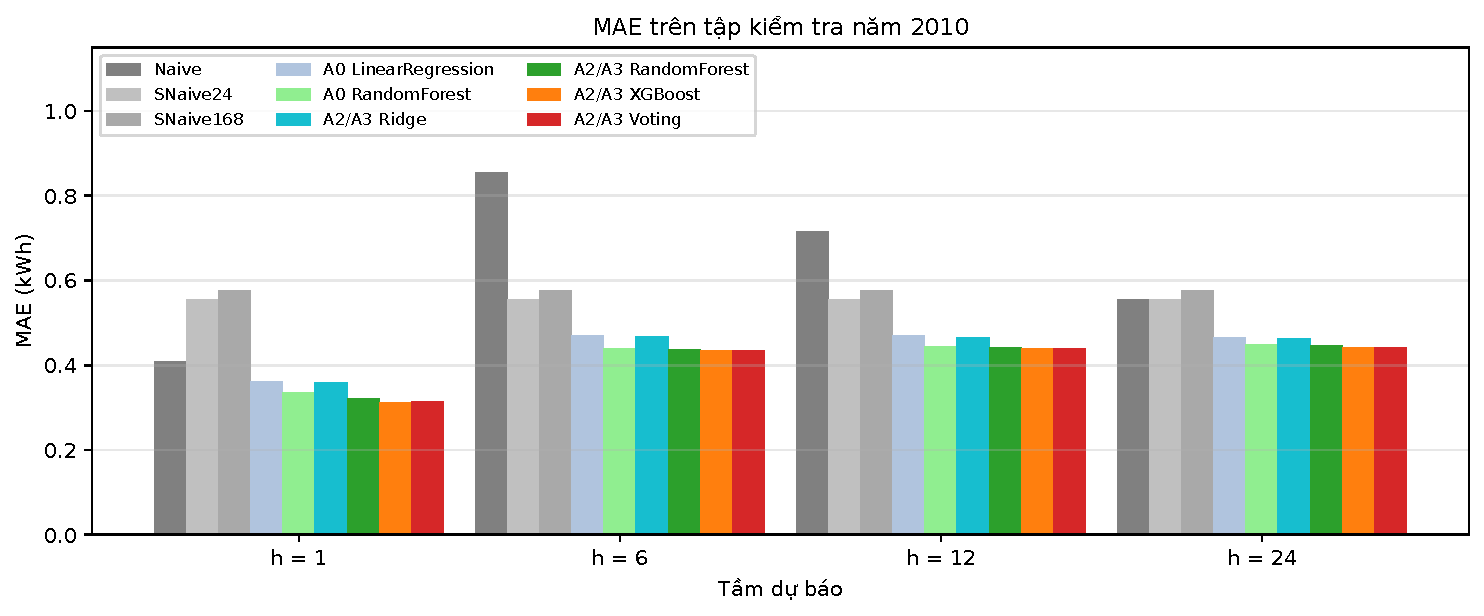
\includegraphics[width=0.92\textwidth]{figures/test_so_sanh.pdf}
    \caption{MAE trên tập kiểm tra năm 2010 của các mô hình.}
    \label{fig:test_compare}
\end{figure}

\paragraph{So với mô hình cơ sở.} Mô hình cuối vượt mọi mô hình cơ sở ở cả bốn tầm dự báo (Bảng~\ref{tab:cv_test}, Hình~\ref{fig:test_compare}): MAE 0,313 kWh ở $h = 1$ và 0,434--0,441 kWh ở $h \ge 6$, thấp hơn 23--25\% so với mô hình cơ sở được chọn trên kiểm định chéo (Naive ở $h = 1$, SNaive168 ở $h \ge 6$). So với mô hình cơ sở tốt nhất trên chính tập kiểm tra (SNaive24, 0,556 kWh ở $h \ge 6$), mức giảm vẫn là 20,6--21,8\%. Mức mong muốn giảm ít nhất 10\% ở mọi $h$ đặt ra ở Bảng~\ref{tab:objectives} vì vậy đạt được cả trên tập kiểm tra. Thứ hạng giữa hai mô hình cơ sở mùa vụ đảo ngược so với kiểm định chéo, cho thấy chênh lệch nhỏ giữa chúng không ổn định qua các giai đoạn.

\paragraph{So với kiểm định chéo.} Thứ hạng các mô hình giữ nguyên: XGBoost đã tối ưu tốt nhất ở mọi $h$, Voting sát sau, Ridge gần như bằng Linear Regression. So với Random Forest của Chương~\ref{chap:models}, mô hình cuối giảm MAE 6,9\% ở $h = 1$ (0,336 xuống 0,313 kWh) và 0,9--1,6\% ở $h \ge 6$, khớp với kết luận của Bảng~\ref{tab:ablation}. MAE trên tập kiểm tra thấp hơn MAE kiểm định chéo (0,313 so với 0,334 kWh ở $h = 1$; 0,441 so với 0,492 kWh ở $h = 24$). Đây không phải dấu hiệu rò rỉ, vì mô hình cơ sở cũng thấp hơn tương tự (Naive 0,408 so với 0,440 kWh; SNaive168 0,577 so với 0,602 kWh): năm 2010 có mức tiêu thụ trung bình thấp hơn (1,055 so với 1,120 kWh ở phần kiểm định của 5 fold) nên dễ dự báo hơn, và mô hình cuối được huấn luyện trên nhiều dữ liệu hơn mọi fold.

\paragraph{Độ ổn định.} Huấn luyện lại mô hình cuối với 5 hạt giống ngẫu nhiên khác nhau cho MAE trên tập kiểm tra dao động rất nhỏ (độ lệch chuẩn 0,0004--0,0008 kWh, chênh lệch lớn nhất 0,0018 kWh). Biến động do tính ngẫu nhiên của thuật toán nhỏ hơn nhiều so với chênh lệch giữa các mô hình và so với biến động giữa các fold (0,05--0,11 kWh), vốn chủ yếu do mùa của giai đoạn kiểm định.

\begin{figure}[htbp]
    \centering
    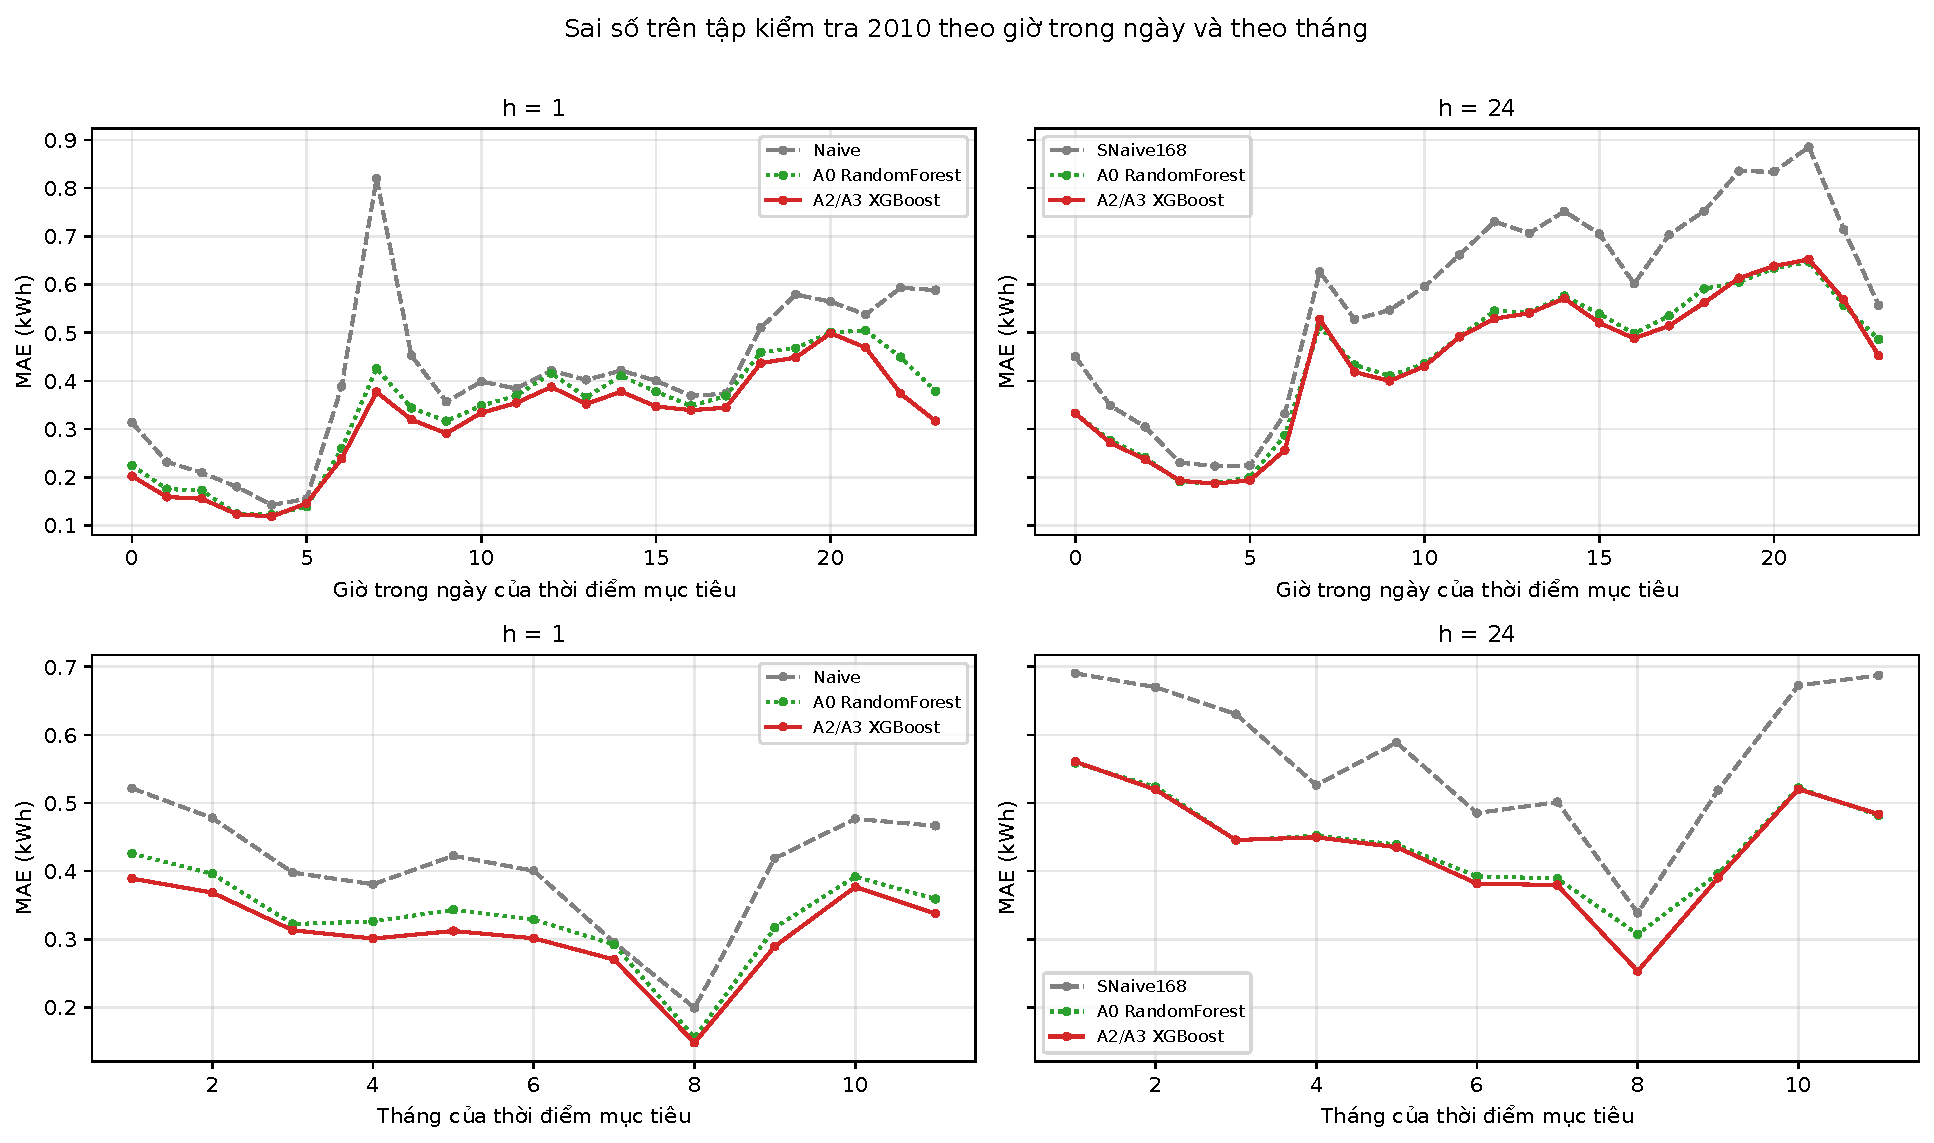
\includegraphics[width=\textwidth]{figures/test_theo_gio_thang.pdf}
    \caption{MAE trên tập kiểm tra theo giờ trong ngày (trên) và theo tháng (dưới) của thời điểm mục tiêu.}
    \label{fig:test_hour_month}
\end{figure}

\paragraph{Sai số theo giờ và theo tháng (Hình~\ref{fig:test_hour_month}).} Mẫu sai số giống kiểm định chéo: thấp nhất lúc 3--4 giờ sáng (khoảng 0,12 kWh ở $h = 1$), cao nhất buổi tối 19--21 giờ (0,45--0,50 kWh ở $h = 1$; 0,61--0,65 kWh ở $h = 24$). Ở $h = 1$, mô hình cuối giảm sai số mạnh nhất lúc 7 giờ sáng so với Naive (0,820 xuống 0,377 kWh); ở $h = 24$, mạnh nhất ở buổi tối so với SNaive168 (21 giờ: 0,885 xuống 0,652 kWh). Theo tháng, sai số cao nhất vào tháng 1 và thấp nhất vào tháng 8. Tháng 8 là trường hợp mô hình cuối kém một mô hình cơ sở ở mọi $h \ge 6$: SNaive24 có MAE 0,188 kWh, còn mô hình cuối 0,229--0,253 kWh (ở $h = 24$ dự báo cao trung bình 0,06 kWh); ở $h = 1$ mô hình cuối vẫn tốt hơn Naive (0,148 so với 0,199 kWh). Tháng 8 tiêu thụ thấp và đều (trung bình 0,51 kWh mỗi giờ được đánh giá), nên lặp lại ngày hôm trước đã rất tốt, còn mô hình học từ cả năm nên kéo dự báo về mức tiêu thụ chung cao hơn.

\paragraph{Giờ đỉnh.} Mô hình cuối vẫn dự báo thấp các giờ đỉnh: ở 5\% giờ tiêu thụ cao nhất của năm 2010 (từ 2,57 kWh), dự báo thấp trung bình 0,90 kWh ở $h = 1$ và 1,32 kWh ở $h = 24$; 10\% số giờ sai nhiều nhất chiếm khoảng 31--35\% tổng sai số tuyệt đối. Mức dự báo thấp ở đỉnh đã giảm so với Bảng~\ref{tab:error_conc} nhưng chưa hết. Hình~\ref{fig:test_week} minh họa: với $h = 1$, mô hình cuối bắt kịp nhiều lần tăng đột ngột sớm hơn Naive, nhưng đỉnh lớn nhất tuần (4,52 kWh lúc 21 giờ ngày 03/02/2010) chỉ được dự báo 2,53 kWh; với $h = 24$, dự báo là một đường trơn tái hiện nhịp tăng buổi sáng và buổi tối hằng ngày nhưng không đoán được các đỉnh riêng lẻ.

\begin{figure}[htbp]
    \centering
    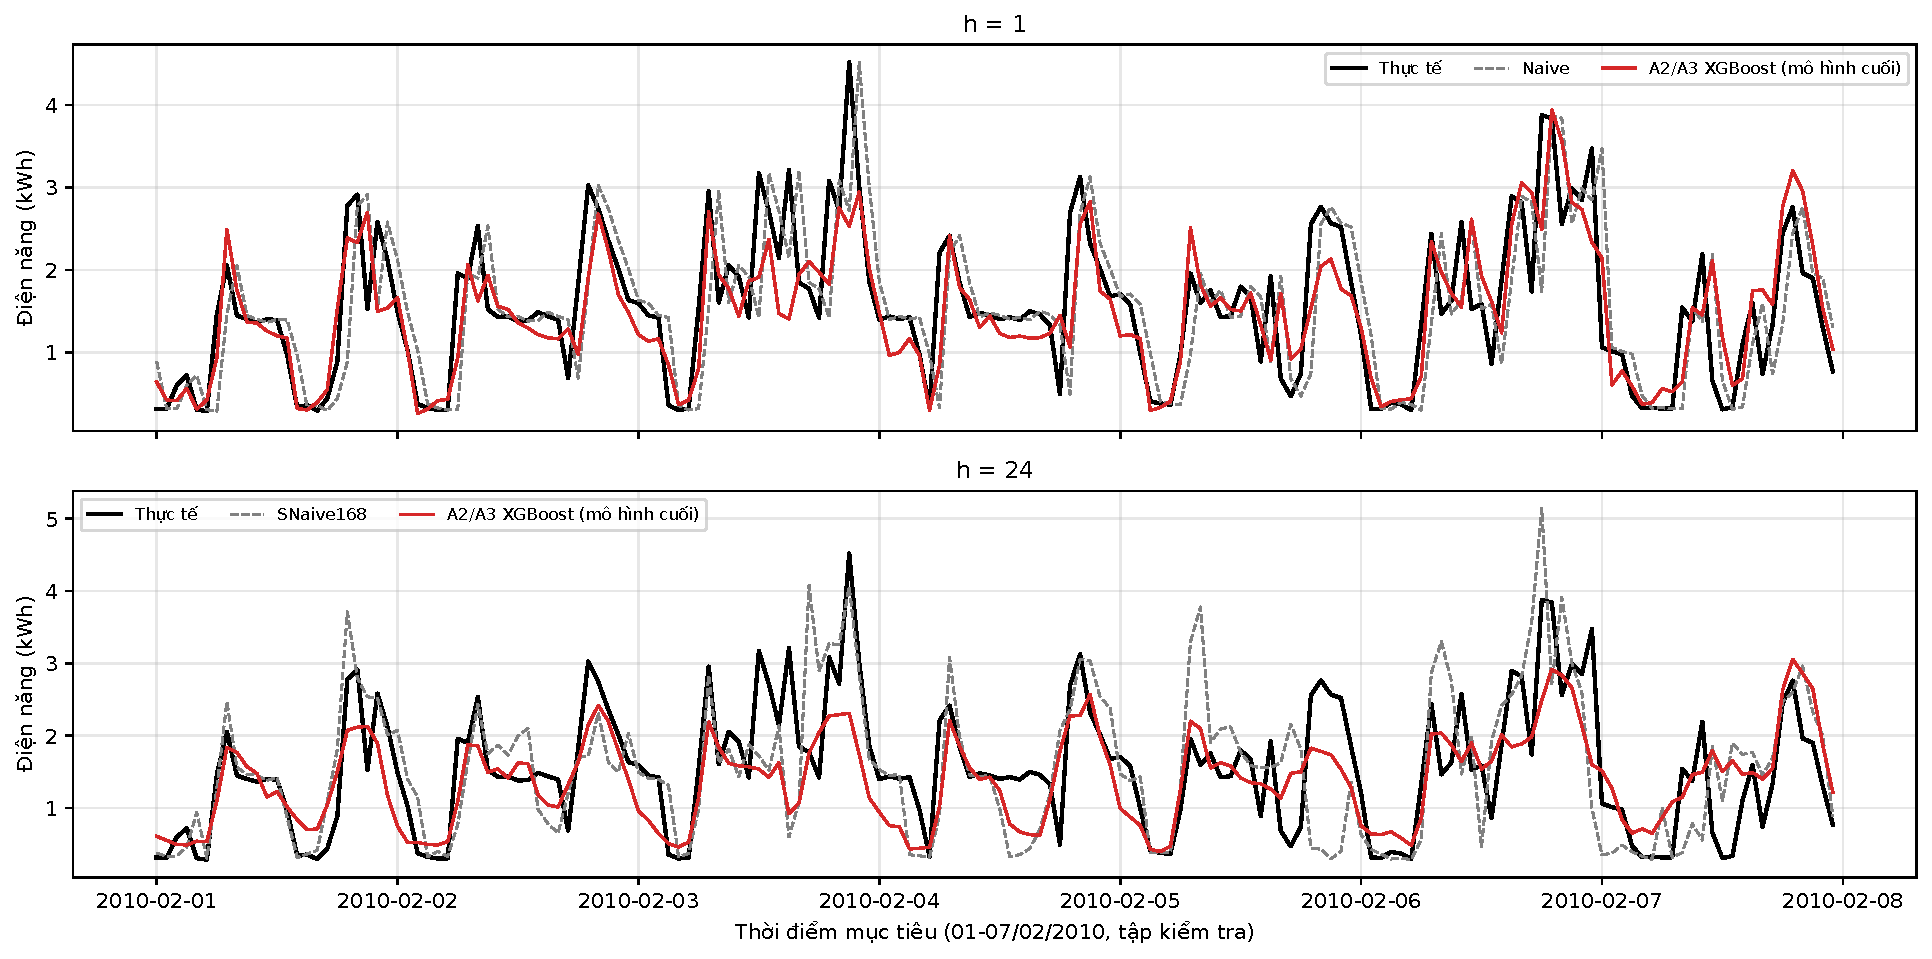
\includegraphics[width=\textwidth]{figures/test_tuan_vi_du.pdf}
    \caption{Dự báo của mô hình cuối và thực tế trong tuần 01--07/02/2010 (tập kiểm tra).}
    \label{fig:test_week}
\end{figure}

\section{Thảo luận}
\label{sec:discussion4}

\paragraph{Vì sao cải tiến có hiệu quả ở $h = 1$ nhưng ít hiệu quả ở $h \ge 6$.} Đường cong kiểm định cho thấy mô hình cây không bị giới hạn bởi phương sai, nên điều chuẩn hay tối ưu siêu tham số chỉ cải thiện rất ít. Mô hình chỉ tốt hơn khi được cung cấp thông tin mới. Thông tin về thiết bị đang chạy có giá trị trong một vài giờ, nên giúp rõ ở $h = 1$ nhưng gần như không giúp ở $h \ge 6$. Ở các tầm dự báo xa, mô hình chủ yếu dựa vào hồ sơ tiêu thụ theo giờ và thứ; phần sai số còn lại đến từ hành vi khó đoán của các thành viên trong hộ, mà dữ liệu điện năng của một hộ không chứa.

\paragraph{Vì sao tổ hợp không giúp.} Kết hợp dự báo thường hiệu quả hơn khi sai số của các mô hình thành phần không tương quan hoàn toàn~\cite{wang2023forecast}. Random Forest và XGBoost dùng cùng đặc trưng và cùng học các quan hệ dạng cây, và cả hai đều dự báo thấp các giờ đỉnh với mức gần nhau (Bảng~\ref{tab:error_conc}); vì vậy lấy trung bình có thể không bù được phần lỗi chung đó.

\paragraph{Ý nghĩa thực tế.} Với mức tiêu thụ trung bình khoảng 1,06 kWh mỗi giờ trong năm 2010, sai số tuyệt đối trung bình 0,31 kWh ở $h = 1$ và khoảng 0,44 kWh ở $h = 24$ đủ để dự báo hồ sơ tiêu thụ trong ngày (giờ thấp điểm, giờ cao điểm buổi sáng và buổi tối), nhưng chưa đủ để dự báo chính xác độ lớn của từng đỉnh tiêu thụ.
